\section{Joomla!}
\label{sec:CMS_joomla}

Joomla is a free and open-source content management system (CMS) for publishing web content. It is built on a model–view–controller web application framework that can be used independently of the CMS. \cite{cms_joomla_overview}

Joomla is written in PHP, uses object-oriented programming (OOP) techniques (since version 1.5  \cite{cms_joomla_mvc}) and software design patterns, stores data in a MySQL, MS SQL (since version 2.5), or PostgreSQL (since version 3.0) database \cite{cms_joomla_2.5}, and includes features such as page caching, RSS feeds, printable versions of pages, news flashes, blogs, search, and support for language internationalization.
As of February 2014, Joomla has been downloaded over 50 million times \cite{cms_joomla_stats}. Over 7,700 free and commercial extensions are available from the official Joomla! Extension Directory, and more are available from other sources. It is estimated to be the second most used content management system on the Internet, after WordPress \cite{cms_stats}. 
Like many other web applications, Joomla may be run on a LAMP stack.
Many web hosts have control panels for automatic installation of Joomla. On Windows, Joomla can be installed using the Microsoft Web Platform Installer, which automatically detects and installs dependencies, such as PHP or MySQL.
Many web sites provide information on installing and maintaining Joomla sites.

\subsection{History}
\label{joomla_his}
Joomla was the result of a fork of Mambo on August 17, 2005. At that time, the Mambo name was a trademark of Miro International Pty Ltd, who formed a non-profit foundation with the stated purpose of funding the project and protecting it from lawsuits. The Joomla development team claimed that many of the provisions of the foundation structure violated previous agreements made by the elected Mambo Steering Committee, lacked the necessary consultation with key stakeholders and included provisions that violated core open source values.
Joomla developers created a website called OpenSourceMatters.org (OSM) to distribute information to the software community. Project leader Andrew Eddie wrote a letter that appeared on the announcements section of the public forum at mamboserver.com. Over one thousand people joined OpenSourceMatters.org within a day, most posting words of encouragement and support. The website received the Slashdot effect as a result. Miro CEO Peter Lamont responded publicly to the development team in an article titled The Mambo Open Source Controversy, 20 Questions With Miro. This event created controversy within the free software community about the definition of open source. Forums of other open-source projects were active with postings about the actions of both sides.
In the two weeks following Eddie's announcement, teams were re-organized and the community continued to grow. Eben Moglen and the Software Freedom Law Center (SFLC) assisted the Joomla core team beginning in August 2005, as indicated by Moglen's blog entry from that date and a related OSM announcement. The SFLC continue to provide legal guidance to the Joomla project.
On August 18, Andrew Eddie called for community input to suggest a name for the project. The core team reserved the right for the final naming decision, and chose a name not suggested by the community. On September 22, the new name, Joomla!, was announced. It is the anglicised spelling of the Swahili word jumla meaning all together or as a whole which also has a similar meaning in at least Amharic, Arabic and Urdu. On September 26, the development team called for logo submissions from the community and invited the community to vote on the logo; the team announced the community's decision on September 29. On October 2, brand guidelines, a brand manual, and a set of logo resources were published.
Joomla won the Packt Publishing Open Source Content Management System Award in 2006, 2007, and 2011 \cite{cms_joomla_overview}.


\subsection{Extensions}
\label{subsec:joomla_ext}
Joomla extensions extend the functionality of Joomla websites. Five types of extensions may be distinguished: components, modules, plugins, templates, and languages. Each of these extensions handles a specific function.
\begin{itemize}
	\item Components are the largest and most complex extensions. Most components have two parts: a site part and an administrator part. Every time a Joomla page loads, one component is called to render the main page body. Components produce the major portion of a page because a component is driven by a menu item.
	\item Plugins are advanced extensions and are, in essence, event handlers. In the execution of any part of Joomla, a module or a component, an event may be triggered. When an event is triggered, plugins that are registered to handle that event execute. For example, a plugin could be used to block user-submitted articles and filter text. The line between plugins and components can sometimes be a little fuzzy. Sometimes large or advanced plugins are called components even though they don't actually render large portions of a page. An SEF URL extension might be created as a component, even though its functionality could be accomplished with just a plugin.
	\item Templates describe the main design of a Joomla website. While the CMS manages the website content, templates determine the style or look and feel and layout of a site.
	\item Modules render pages in Joomla. They are linked to Joomla components to display new content or images. Joomla modules look like boxes, such as the search or login module. However, they don’t require html in Joomla to work.
	\item Languages are very simple extensions that can either be used as a core part or as an extension. Language and font information can also be used for PDF or PSD to Joomla conversions \cite{cms_joomla_overview}.
\end{itemize}




\begin {figure}[h]
\graphicspath{{images/chapter_cms/}}
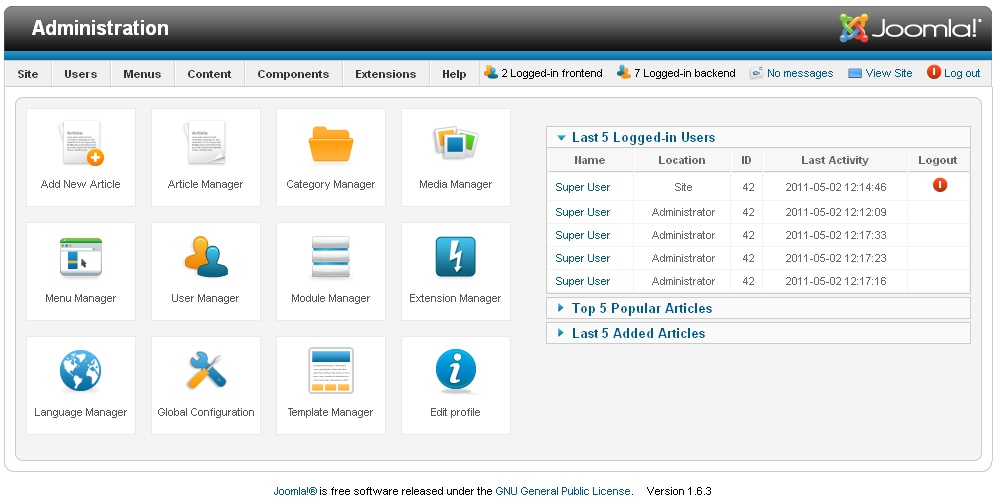
\includegraphics[width=\textwidth]{joomla_dash}
\caption{Joomla! Dashboard}
\end {figure}
